\documentclass{beamer}

%%% ISSUE BBB solved %%%
%\usepackage{lmodern}
%%%%%%%%%%%%%%%%%%%%%%%%

\usepackage[utf8]{inputenc}
\usepackage[T1]{fontenc}
\usepackage{multicol}
\usepackage{amsthm}
\usepackage{amsmath}
\usepackage{amssymb}
\usepackage{mathtools}
\usepackage{dsfont}
\usepackage{bm}
\usepackage{bbm}
\usepackage{xparse}
\usepackage{physics}
\usepackage{empheq}
\usepackage{url}
\usepackage{hyperref}
%\usepackage[affil-it]{authblk}
%\usepackage{enumitem}
\usepackage{rotating}
\usepackage{graphicx}
\usepackage[linesnumbered,ruled,vlined]{algorithm2e}

\usepackage{tikz}
\usetikzlibrary{calc}
\usetikzlibrary{shapes,arrows}

\tikzstyle{block} = [draw, fill=white, rectangle, 
  minimum height=2em, minimum width=3em]
\tikzstyle{bigblock} = [draw, fill=white, rectangle, 
  minimum height=3em, minimum width=4em]
\tikzstyle{Bigblock} = [draw, fill=white, rectangle, 
    minimum height=5em, minimum width=8.5em]
\tikzstyle{input} = [coordinate]
\tikzstyle{output} = [coordinate]
\tikzstyle{pinstyle} = [pin edge={to-,thin,black}]

\usepackage{pgfplots}
\pgfplotsset{compat = newest}

\theoremstyle{definition}
\newtheorem{theo}{Theorem}[section]
\newtheorem{lem}[theo]{Lemma}
\newtheorem{cor}[theo]{Corollary}
\newtheorem{prop}[theo]{Proposition}
\newtheorem{defi}[theo]{Definition}
\newtheorem{conj}[theo]{Conjecture}

\newtheorem{theo*}{Theorem}

\theoremstyle{remark}
\newtheorem*{rk}{Remark}

\DeclareMathOperator{\Poi}{\text{Poi}}
\DeclareMathOperator{\Ber}{\text{Ber}}
\DeclareMathOperator{\Bin}{\text{Bin}}
\DeclareMathOperator{\maxi}{\text{maximize}}
\DeclareMathOperator{\mini}{\text{minimize}}
\DeclareMathOperator{\st}{\text{subject to}}
\DeclarePairedDelimiter\ceil{\lceil}{\rceil}
\DeclarePairedDelimiter\floor{\lfloor}{\rfloor}
\DeclarePairedDelimiterX\set[1]\lbrace\rbrace{\def\given{\;\delimsize\vert\;}#1}

\colorlet{darkgreen}{green!40!black}

\usepackage{appendixnumberbeamer}
\beamertemplatenavigationsymbolsempty

%%%%%%%%%
\usetheme{Dresden}
\usecolortheme{lily}
\newcommand*\oldmacro{}%
\let\oldmacro\insertshorttitle%
\renewcommand*\insertshorttitle{%
  \oldmacro\hfill%
  \insertframenumber\,/\,\inserttotalframenumber}
%%%%%%%%%



\title{Approximation Algorithms for Channel Coding and Non-Signaling Correlations}
\subtitle{\textit{Algorithmes d'approximation pour le problème du codage de canal et corrélations non-signalantes}}
\author{Paul Fermé}
\institute{ENS de Lyon}
\date{29 novembre 2023}

%\AtBeginSection[]
%{
%  \begin{frame}<beamer>
%    \frametitle{Contents}
%    \tableofcontents[currentsection]
%  \end{frame}
%}

%%%%%%%%%%%%%%%%%%%%%%%%%%%%%%%%%%%%%%%%%%
\begin{document}
%%%%%%%%%%%%%%%%%%%%%%%%%%%%%%%%%%%%%%%%%%

\begin{frame}
  \titlepage
\end{frame}


\section{Introduction}
\begin{frame}{Qu'est ce qu'un canal de communication ?}
  \pause
  \begin{center}
    \includegraphics[scale=0.42]{tin-can-telephone.jpg}
    
      \pause
      Vent ? Pluie ? Obstacles ?
  \end{center}
\end{frame}

\begin{frame}{Communiquer avec du bruit ?}
  \begin{center}
  \begin{tikzpicture}
    %%% Tin can telephone %%%
    \node at (4.7,0) (tin) {\includegraphics[scale=0.22]{long-tin-can-telephone.jpg}};

    %%% Left callouts %%%
    \only<1-2>{\node[ellipse callout, draw, callout relative pointer={(-0.3,-0.3)}] at (-0.1,0.1) (Alice) {\Large Allô!};}
    \only<3>{\node[ellipse callout, draw, callout relative pointer={(-0.3,-0.3)}] at (-0.1,2.1) (Alice) {\Large \alert{A}llô!};
      \node[ellipse callout, draw, callout absolute pointer={(-0.1,1.5)}] at (-0.1,0.1) (Alice) {Alfa};}
    \only<4>{\node[ellipse callout, draw, callout relative pointer={(-0.3,-0.3)}] at (-0.1,2.1) (Alice) {\Large A\alert{l}lô!};
      \node[ellipse callout, draw, callout absolute pointer={(-0.1,1.5)}] at (-0.1,0.1) (Alice) {Lima};}
    \only<5>{\node[ellipse callout, draw, callout relative pointer={(-0.3,-0.3)}] at (-0.1,2.1) (Alice) {\Large Al\alert{l}ô!};
      \node[ellipse callout, draw, callout absolute pointer={(-0.1,1.5)}] at (-0.1,0.1) (Alice) {Lima};}
    \only<6>{\node[ellipse callout, draw, callout relative pointer={(-0.3,-0.3)}] at (-0.1,2.1) (Alice) {\Large All\alert{ô}!};
      \node[ellipse callout, draw, callout absolute pointer={(-0.1,1.5)}] at (-0.1,0.1) (Alice) {\small Oscar};}
    %%% Cloud %%%
    \only<1>{\node at (4.6,1.5) (wcloud) {\includegraphics[scale=0.3]{rcloud_white.png}};}
    \only<2-6>{\node at (4.6,1.5) (cloud) {\includegraphics[scale=0.3]{rcloud.png}};}

    %%% Right callouts %%%
    \only<1>{\node[ellipse callout, draw, callout relative pointer={(-0.2,0)}] at (9.7,0.1) (Bob) {\Large Allô!};}
    \only<2>{\node[dashed, ellipse callout, draw, callout relative pointer={(-0.2,0)}] at (9.7,0.1) (Bob) {\tiny Ah, l'eau!};}
    \only<3>{\node[dashed, ellipse callout, draw, callout relative pointer={(-0.2,0)}] at (9.4,0.1) (Bob) {\tiny Alma};
      \node[ellipse callout, draw, callout absolute pointer={(9.4,0.5)}] at (9.4,2.1) (Alice) {\Large \alert{A}};}
    \only<4>{\node[dashed, ellipse callout, draw, callout relative pointer={(-0.2,0)}] at (9.4,0.1) (Bob) {\tiny Lena};
      \node[ellipse callout, draw, callout absolute pointer={(9.4,0.5)}] at (9.4,2.1) (Alice) {\Large A\alert{L}};}
    \only<5>{\node[dashed, ellipse callout, draw, callout relative pointer={(-0.2,0)}] at (9.4,0.1) (Bob) {\tiny Rima};
      \node[ellipse callout, draw, callout absolute pointer={(9.4,0.5)}] at (9.4,2.1) (Alice) {\Large AL\alert{L}};}
    \only<6>{\node[dashed, ellipse callout, draw, callout relative pointer={(-0.2,0)}] at (9.5,0.1) (Bob) {\tiny Lascar};
      \node[ellipse callout, draw, callout absolute pointer={(9.5,0.5)}] at (9.5,2.1) (Alice) {\Large ALL\alert{O}};}
  \end{tikzpicture}
  \end{center}
\end{frame}


\begin{frame}{Modélisation mathématique}
  \begin{center}
    \begin{tikzpicture}[auto, node distance=2cm,>=latex']
      \node [bigblock] (W) {\only<1-2>{$W$}\only<3>{$6/10$}\only<4>{$3/10$}\only<5>{$1/10$}};
      \node [right of=W] (y) {\only<1-2>{$y$}\only<3>{\emph{alfa}}\only<4>{\emph{alma}}\only<5>{\emph{alvo}}};
      \node [left of=W] (x) {\only<1-2>{$x$}\only<3-5>{\emph{alfa}}};
      \draw [->] (x) -- (W);
      \draw [->] (W) -- (y);
    \end{tikzpicture}

    \pause
    \bigskip
    Probabilité \only<2>{$W(y|x)$}\only<3>{$6/10$}\only<4>{$3/10$}\only<5>{$1/10$} d'avoir la sortie \only<2>{$y$}\only<3>{\emph{alfa}}\only<4>{\emph{alma}}\only<5>{\emph{alvo}} pour l'entrée \only<2>{$x$}\only<3-5>{\emph{alfa}}
  \end{center} 
\end{frame}

\begin{frame}{Le problème du codage de canal}
  \begin{center}
    \begin{tikzpicture}[auto, node distance=2.5cm,>=latex']
      \node [block] (e) {$e$};
      \node [bigblock, right of=e] (W) {\only<1,5>{$W$}\only<2>{$6/10$}\only<3>{$3/10$}\only<4>{$1/10$}};
      \node [block, right of=W] (d) {$d$};
      \draw [->] (e) -- node[name=x] {\only<1,5>{$x$}\only<2-4>{\emph{alfa}}} (W);
      \draw [->] (W) -- node[name=y] {\only<1,5>{$y$}\only<2>{\emph{alfa}}\only<3>{\emph{alma}}\only<4>{\emph{alvo}}} (d);
      \node [left of=e, node distance=1.5cm] (i) {\only<1>{$i$}\only<2-4>{\alert{a}}\only<5>{\alert{b,\ldots,z}}};
      \node [right of=d,  node distance=1.5cm] (j) {\only<1>{$j$}\only<2-3>{\alert{a}}\only<4>{\alert{b}}\only<5>{\alert{b,\ldots,z}}};
      \draw [draw,->] (i) -- (e);
      \draw [draw,->] (d) -- (j);
    \end{tikzpicture}

    \bigskip

    Trouver $e$ et $d$ qui maximise la probabilité d'avoir $j=i$\only<5>{\ldots\\
      \bigskip
      \ldots sur tout l'alphabet (noté $[k]$; ici $k=26$) ! Formellement:
      \[ \underset{e,d}{\max} \ \frac{1}{k} \sum_{i,x,y} e(x|i)W(y|x)d(i|y) \]
    }
  \end{center}
\end{frame}

\begin{frame}{Résolution \cite{BF18}}
  \begin{itemize}
  \item \underline{Objectif:} méthode systématique (algorithme) pour trouver les meilleurs $e,d$ pour un $W$.
    \pause
  \item \underline{Problème:} impossible (\textrm{NP}-difficulté) de créer un algorithme efficace (temps polynomial) qui trouve ces $e,d$.
    \bigskip
    \pause
  \item \underline{Solution:} plutôt que les meilleurs $e,d$, on se contente d'un choix de $e,d$ avec une valeur \emph{proche} des meilleurs.
    
    \pause
    \bigskip

  \item \cite{BF18}: approximation qui garantit au moins $\simeq 63\%$ (coefficient $1-e^{-1}$) aussi bien que les meilleurs.
  \item Impossible (\textrm{NP}-difficile) de faire mieux que $1-e^{-1}$.
  \end{itemize}
\end{frame}

\begin{frame}{Décodage de liste}
  \begin{center}
    \begin{tikzpicture}[auto, node distance=2.5cm,>=latex']
      \node [block] (e) {$e$};
      \node [bigblock, right of=e] (W) {\only<1,3-6>{$W$}\only<2>{$1/10$}};
      \node [block, right of=W] (d) {$d$};
      \draw [->] (e) -- node[name=x] {\only<1,3-6>{$x$}\only<2>{\emph{alfa}}} (W);
      \draw [->] (W) -- node[name=y] {\only<1,3-6>{$y$}\only<2>{\emph{alvo}}} (d);
      \node [left of=e, node distance=1.5cm] (i) {\only<1,3-6>{$i$}\only<2>{\alert{a}}};
      \node [right of=d,  node distance=2cm] (j) {\only<1>{$[j_1,j_2]$}\only<2>{\alert{[a,b]}}\only<3-6>{$[j_1,j_2,\ldots,j_{\ell}]$}};
      \draw [draw,->] (i) -- (e);
      \draw [draw,->] (d) -- (j);
    \end{tikzpicture}

    \bigskip
    Trouver $e,d$ qui maximise la probabilité que \only<1-2>{$j_1$ ou $j_2$}\only<3-6>{$j_1,j_2,\ldots$ ou $j_{\ell}$} égal à $i$.
  \end{center}
  
  \pause\pause\pause
  
  \begin{itemize}
  \item \cite{BFGG20}: Algorithme d'approximation avec un facteur $1-\frac{\ell^{\ell}e^{-\ell}}{\ell!}$ (pour $\ell=2$, correspond à $\simeq 73\%$).
    \pause
  \item On va montrer que c'est \textrm{NP}-difficile de faire mieux.
    \pause
  \item On va étudier une généralisation, où la taille $\ell$ de la liste n'est pas fixée, mais vient avec une pénalité $\frac{\varphi(\ell)}{\ell}$.
  \end{itemize}
\end{frame}

\begin{frame}{Le cantique des quantiques}

\end{frame}
%%%%%%%%%%%%%%%%%%%%%%%%%%%%%%%%%%%%%%%%%%
\section{Bibliography}
\begin{frame}[allowframebreaks]{Bibliography}
  \bibliographystyle{alphaurl}
  \bibliography{these}
\end{frame}
%%%%%%%%%%%%%%%%%%%%%%%%%%%%%%%%%%%%%%%%%%

%%%%%%%%%%%%%%%%%%%%%%%%%%%%%%%%%%%%%%%%%%
\end{document}
%%%%%%%%%%%%%%%%%%%%%%%%%%%%%%%%%%%%%%%%%%
